%%
%% This is file `sample-sigconf.tex',
%% generated with the docstrip utility.
%%
%% The original source files were:
%%
%% samples.dtx  (with options: `sigconf')
%% 
%% IMPORTANT NOTICE:
%% 
%% For the copyright see the source file.
%% 
%% Any modified versions of this file must be renamed
%% with new filenames distinct from sample-sigconf.tex.
%% 
%% For distribution of the original source see the terms
%% for copying and modification in the file samples.dtx.
%% 
%% This generated file may be distributed as long as the
%% original source files, as listed above, are part of the
%% same distribution. (The sources need not necessarily be
%% in the same archive or directory.)
%%
%%
%% Commands for TeXCount
%TC:macro \cite [option:text,text]
%TC:macro \citep [option:text,text]
%TC:macro \citet [option:text,text]
%TC:envir table 0 1
%TC:envir table* 0 1
%TC:envir tabular [ignore] word
%TC:envir displaymath 0 word
%TC:envir math 0 word
%TC:envir comment 0 0
%%
%%
%% The first command in your LaTeX source must be the \documentclass command.
\documentclass[sigconf,authorversion,noacm]{acmart}
\settopmatter{printacmref=false}

%%
%% \BibTeX command to typeset BibTeX logo in the docs
\AtBeginDocument{%
  \providecommand\BibTeX{{%
    Bib\TeX}}}

%% Rights management information.  This information is sent to you
%% when you complete the rights form.  These commands have SAMPLE
%% values in them; it is your responsibility as an author to replace
%% the commands and values with those provided to you when you
%% complete the rights form.

%% These commands are for a PROCEEDINGS abstract or paper.


%%
%% Submission ID.
%% Use this when submitting an article to a sponsored event. You'll
%% receive a unique submission ID from the organizers
%% of the event, and this ID should be used as the parameter to this command.
%%\acmSubmissionID{123-A56-BU3}

%%
%% For managing citations, it is recommended to use bibliography
%% files in BibTeX format.
%%
%% You can then either use BibTeX with the ACM-Reference-Format style,
%% or BibLaTeX with the acmnumeric or acmauthoryear sytles, that include
%% support for advanced citation of software artefact from the
%% biblatex-software package, also separately available on CTAN.
%%
%% Look at the sample-*-biblatex.tex files for templates showcasing
%% the biblatex styles.
%%

%%
%% The majority of ACM publications use numbered citations and
%% references.  The command \citestyle{authoryear} switches to the
%% "author year" style.
%%
%% If you are preparing content for an event
%% sponsored by ACM SIGGRAPH, you must use the "author year" style of
%% citations and references.
%% Uncommenting
%% the next command will enable that style.
%%\citestyle{acmauthoryear}



%%
%% end of the preamble, start of the body of the document source.
\begin{document}

%%
%% The "title" command has an optional parameter,
%% allowing the author to define a "short title" to be used in page headers.
\title{Improving cache allocation for networked applications using unikernels}

%%
%% The "author" command and its associated commands are used to define
%% the authors and their affiliations.
%% Of note is the shared affiliation of the first two authors, and the
%% "authornote" and "authornotemark" commands
%% used to denote shared contribution to the research.
\author{Jiangqiong Liu}
\email{liu3328@purdue.edu}
\affiliation{
    \institution{Purdue University}
    \country{United States}}

\author{Joshua Reprogle}
\email{jreprogl@purdue.edu}
\affiliation{
    \institution{Purdue University}
    \country{United States}}

\author{Vedaant Rajoo}
\email{vrajoo@purdue.edu}
\affiliation{
    \institution{Purdue University}
    \country{United States}}

\author{Sowmya Jayaram Iyer}
\email{jayarami@purdue.edu}
\affiliation{
    \institution{Purdue University}
    \country{United States}}

\author{Keerthana Ashokkumar}
\email{kashokku@purdue.edu}
\affiliation{
    \institution{Purdue University}
    \country{United States}}

\author{Anmol Sahoo}
\affiliation{
    \institution{Purdue University}
    \country{United States}}
\email{sahoo9@purdue.edu}

%%
%% By default, the full list of authors will be used in the page
%% headers. Often, this list is too long, and will overlap
%% other information printed in the page headers. This command allows
%% the author to define a more concise list
%% of authors' names for this purpose.
\renewcommand{\shortauthors}{Liu et al.}

%%
%% The abstract is a short summary of the work to be presented in the
%% article.
\begin{abstract}
In this project, we intend to use unikernels to improve the performance of
networked applications. Since networked applications contend heavily for
scarce CPU resources such as caches, memory bandwidth and compute units,
precise hardware resource allocation is difficult to perform for each
application. Thus, we propose to use unikernels which only bring the minimal
amount of code required to run the application and hope to demonstrate that
this would improve resource utilization in the processor. We intend to use
the Unikraft unikernel framework and deploy applications on the Firecracker
VMM. We will implement our resource allocation policy in Firecracker and use
Unikraft to develop some representative workloads across machine learning,
distributed systems and control plane applications and then present the
effectiveness of our results.
\end{abstract}

\maketitle

\section{Introduction}

As networking interfaces start breaking the 100-Gbps barrier, it is being
observed that commodity processors are not able to keep up with processing
packets at the rate required to saturate these links. With the end of Moore's
law and Dennard scaling, there is an upper limit to how many instructions can be
processed in a given interval, thus limiting the bandwidth achievable on
commodity processors. This is further exacerbated by the fact that memory speeds
have stayed mostly constant, thus main memory access is the critical bottleneck
to processing packets at fast rates. To deal with this problem, modern
processors often include features implementing Direct Cache Access (DCA) which
allows peripheral devices to directly read and write data from the last-level
cache of the processor. Since the peripheral can bypass the entire main memory,
this reduces the effect of the slow memory hierarchy on the packet processing
critical path and provides a pathway to better performance, at least on paper.
But the presence of DCA does not necessarily improve performance and in certain
cases may even decrease performance. Typically, since caches are small and there
is high contention for cache space, DCA may not be able to place packets
efficiently in the cache. A thorough study of the effects of DCA on networked
applications is provided in \cite{alireza_2020}. While existing solutions to
this problem rely on using coarse grained cache partitioning to isolate
different applications, they do not consider the cache contention arising from
\textit{within} an application. As we know, the computational and networking
parts of the applications may have different cache footprints and thus limit the
effectiveness of DCA, since they are both competing for cache resources. To
tackle this problem, we develop a solution based on two key insights - (1)
intra-application cache partitioning and (2) unikernels. We show that these two
insights together are necessary to achieve a holistic solution that reduces the
effects of cache contention arising from different parts of the same
application. Concretely, we implement a system within a hypervisor (KVM) that
allows an application to signal when it wants to switch into code that performs
networking. The hypervisor uses this to information to partition the cache using
Intel Resource Director Technology (RDT). Using this interface, we write various
applications that are bundled with platform code to form a unikernel (Unikraft)
and then deploy it on an Intel CPU supporting Intel RDT. Finally, we use perf to
capture hardware events and measure the change in performance. While results
look promising for some benchmarks ($\sim$10$\%$ improvement in runtime), they
are not consistent across our entire testset. We identify areas of improvement
which can make this solution feasible in practice.

\section{Background and Motivation}

Peripheral devices rely on the use of Direct Memory Access (DMA) to perform IO
operations. DMA technology implemented in processors allows peripheral devices
to directly write to system main memory through the Peripheral Component
Interface-express (PCIe) bus.
The typical flow of a network interface card (NIC) peripheral to receive a
packet is to write the incoming packet in main memory and then signal the
processor via an interrupt about this event. The processor may then perform
additional processing on the packet, write a new packet to main memory and then
signal the NIC to send it out.
Thus, we can see why the memory is a bottleneck in this situation. At 100Gbps, a
processor has 6.72ns to process small packets. But a memory access on the order
of 100ns, makes this prohibitive. To address this problem processors implement
Direct Cache Access (DCA) technology. DCA is an umbrella term to refer to
technologies that can used to improve access time of peripheral DMA data, by
placing it in the cache.
For example, a simple technique allows a cache prefetcher to prefetch parts of
the peripheral memory, thus improving access in predictable scenarios. Intel
processors implement a DCA feature named DDIO (Direct-Data IO). In this setup, a
NIC can perform DMA directly from/to the cache bypassing the main memory
altogether. This prevents the delay incurred by the processor accessing the
packet from main memory. Similarly, while writing the packet the NIC can read
the packet from the cache, avoiding the latency of the main memory. We describe
this process in detail, as it highlights the role that cache contention plays in
this situation. When a NIC receives a packet, it writes a cache line (memory
address block) into the LLC via PCIe. In this case, DDIO overwrites the cache
line if it is present in the cache (PCIe write hit / write update) or allocates
a new line if not (PCIE write miss / write allocate). Note that in the first
case, DDIO may write the packet anywhere in the cache but in the second case, it
may only allocate a packet in a specific region of the cache implying that
frequent write allocations will not make effective use of the cache. When the
processor signals the NIC to send a cache line containing the packet, the NIC
will direcly read the packet from the cache using DDIO. Similar to the previous
case, if the cache line is present in the cache then it is a hit (PCIe read hit)
otherwise it reads the cache line from main memory (PCIe read miss). With this,
it becomes possible to see how DDIO may be affected by cache contention. The
first problem is called leaky DMA \cite{tootoonchian-resq}, where incoming
packets arrive faster than they can be processed thus evicting older packets
from memory. While one solution to this is to limit the number of RX descriptors
(so that the cache space used by DDIO is bounded) it is only a temporary patch.
Small number of RX descriptors increases the packet loss, since fewer packets
can be buffered now. Similarly, limiting TX descriptors is also another proposed
solution, but reducing the number of TX descriptors leads to inefficient
utilization of the PCIe bandwidth. Thus, both of these problems are mitigated by
increasing the number of RX/TX descriptors, but this then overloads the cache
and leads to reduced DDIO efficiency. Along the same lines, cache contention can
lead to eviction of RX/TX buffers, thus if a networked application is also
performing some non-trivial computation, DDIO efficiency is affected. Along the
same lines, cache contention between different parts of the application can also
evict these buffers. Thus, we focus on the problem of solving cache-contention
between different parts of the application with the intention of improving
network performance. We provide a simple motivating example in
Fig.1. As can be seen in Fig.1(a), at a certain point in the program's call
stack, the cache is occupied by the packets that were received due to network
IO. Now, the application executes some computation which displaces these cache
lines, as seen in Fig.1(b). Now any future network IO that may need to be
performed on these packets, would need to fetch them from main memory again.
This clearly highlights the problem of different parts of the application
contending for cache memory and thus affecting networking performance.

\begin{figure}[h]
  \centering
  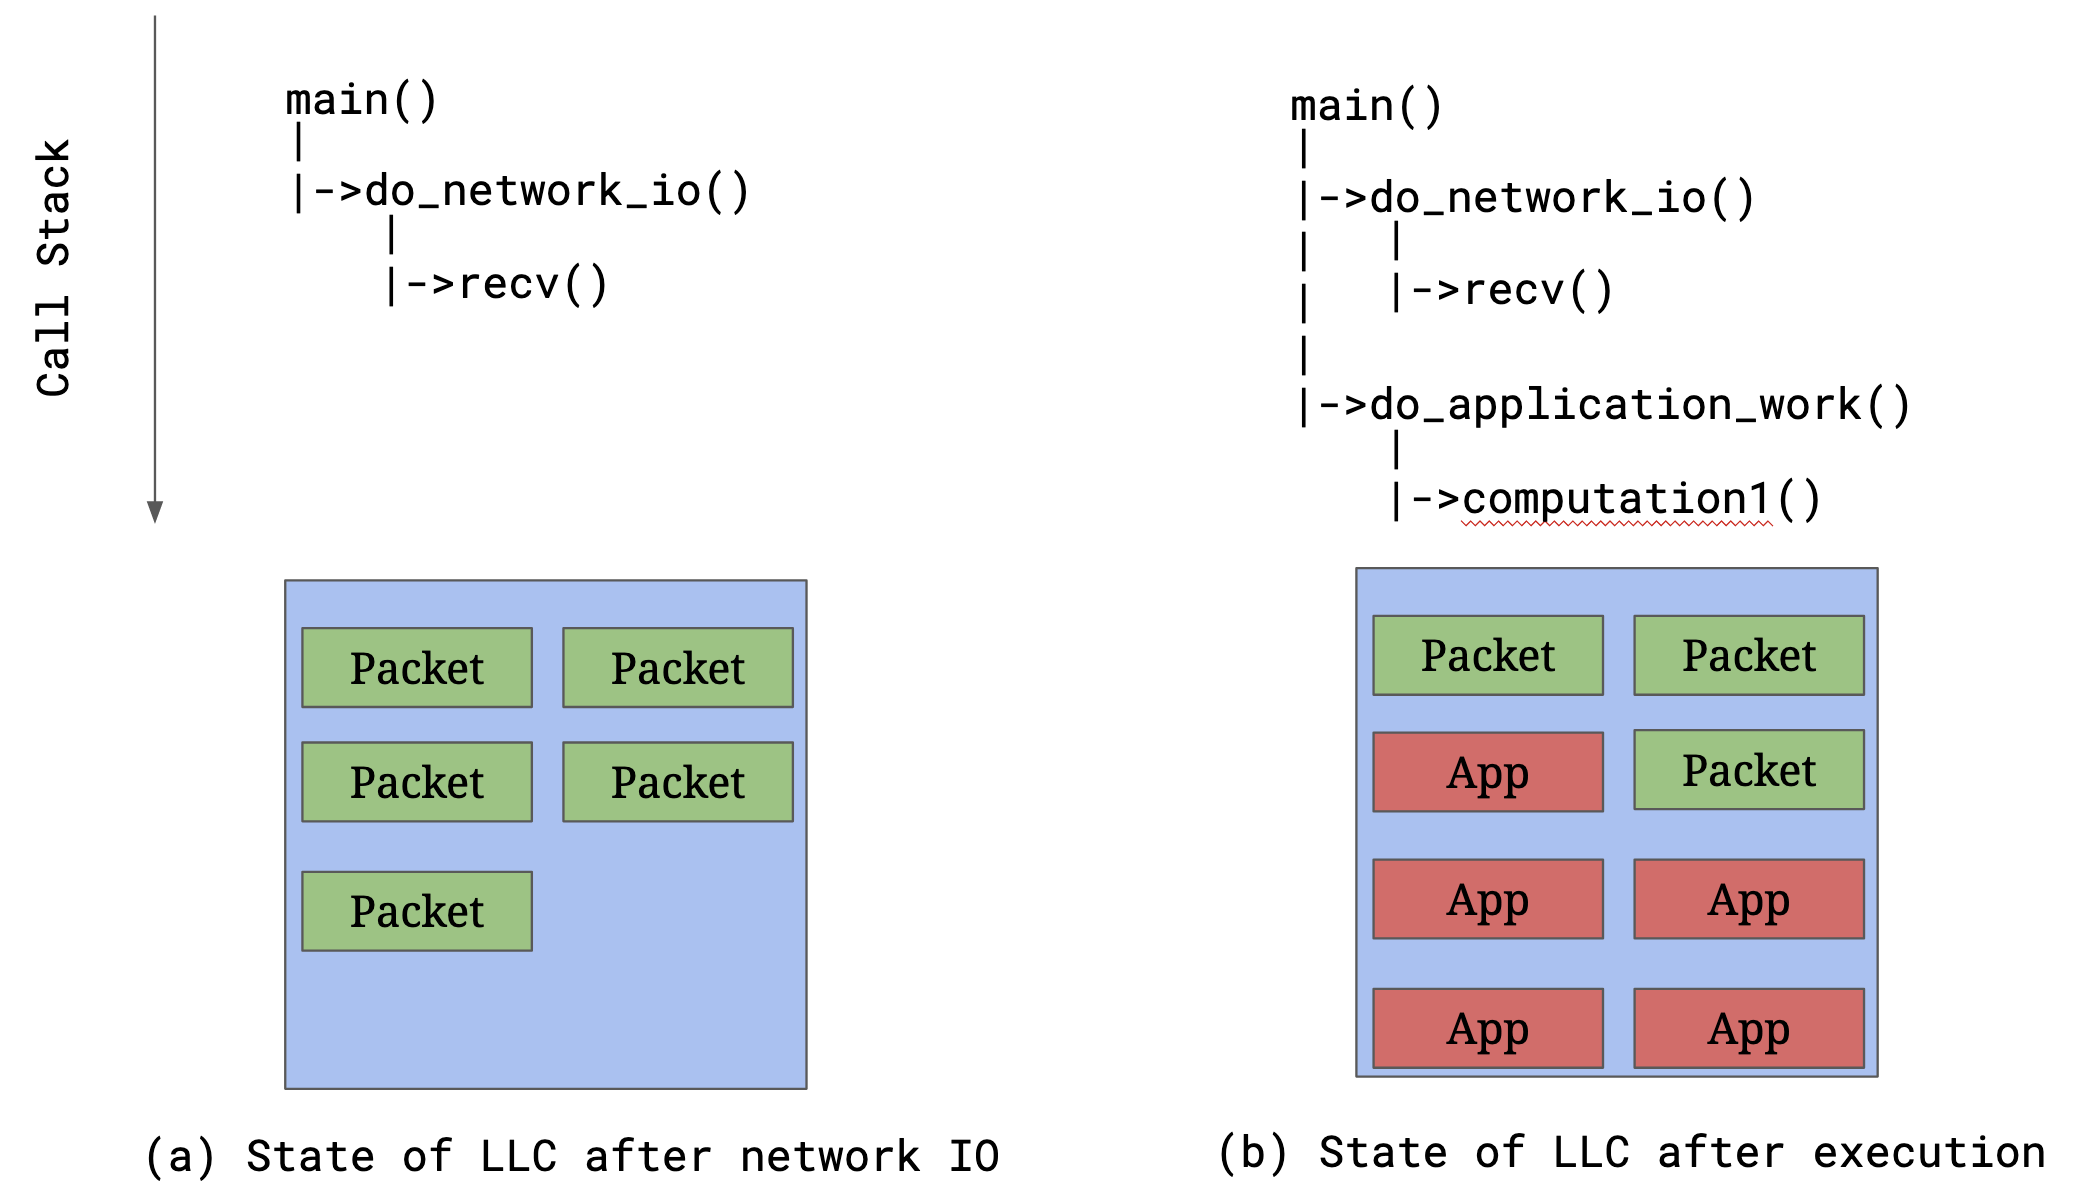
\includegraphics[width=\linewidth]{motivating_example}
    \label{fig:motivating}
    \caption{Motivating Example}
    \Description{Brief representation of our contributions at different layers.
    Boxes in green represent our contribution and boxes in grey are the existing
    systems that are being reused}
\end{figure}

\section{Proposed Solution}

To mitigate the problems that we discussed in Section 2, we develop our solution
based on two key insights - (1) intra-application cache partitioning and (2)
using unikernels to remove OS contention. Intra-application cache partitioning
refers to a technique whereby we perform fine-grained partitioning of the cache,
such that different parts of the same application occupy different parts of the
cache, thus reducing cache contention. By isolating the parts of the cache in
which the RX/TX buffers reside, interference from different parts of the
application are prevented. Thus, these buffers are not evicted and DDIO
performance is not affected. The second idea of using a unikernel is to reduce
interference from the Operating System (OS). An Operating System (OS) is
responsible for providing an abstraction of the CPU for applications. It
maintains multiple in-memory structures for providing various services such as
scheduling, virtual memory, device IO and others. While this is necessary for
enabling multi-user interactive systems (such as terminals), running specialized
applications such as networking services do not require these features. Further,
applications running on hypervisors face a duplication in abstraction layers,
because the same abstractions are provided at both OS and hypervisor layer
(though this can be offset with hardware acceleration such as KVM and SRIOV).
But, the most important problem with an OS in the context of intra-application
cache partitioning is that it renders any analysis of the application useless.
When an application switches into a cache partition, it maybe preempted by the
OS at any point of time. Now, the OS needs to switch its cache partition but it
may still interfere with the memory buffers of the application (through cache
flushes). Thus, even an effective intra-application partitioning scheme would
not be useful in the presence of an OS. This overhead is mitigated by using
unikernels, which offset the interference caused by the OS, since they are
specialized kernels which bundle only the necessary platform code to run the
application.

\begin{figure}[h]
  \centering
  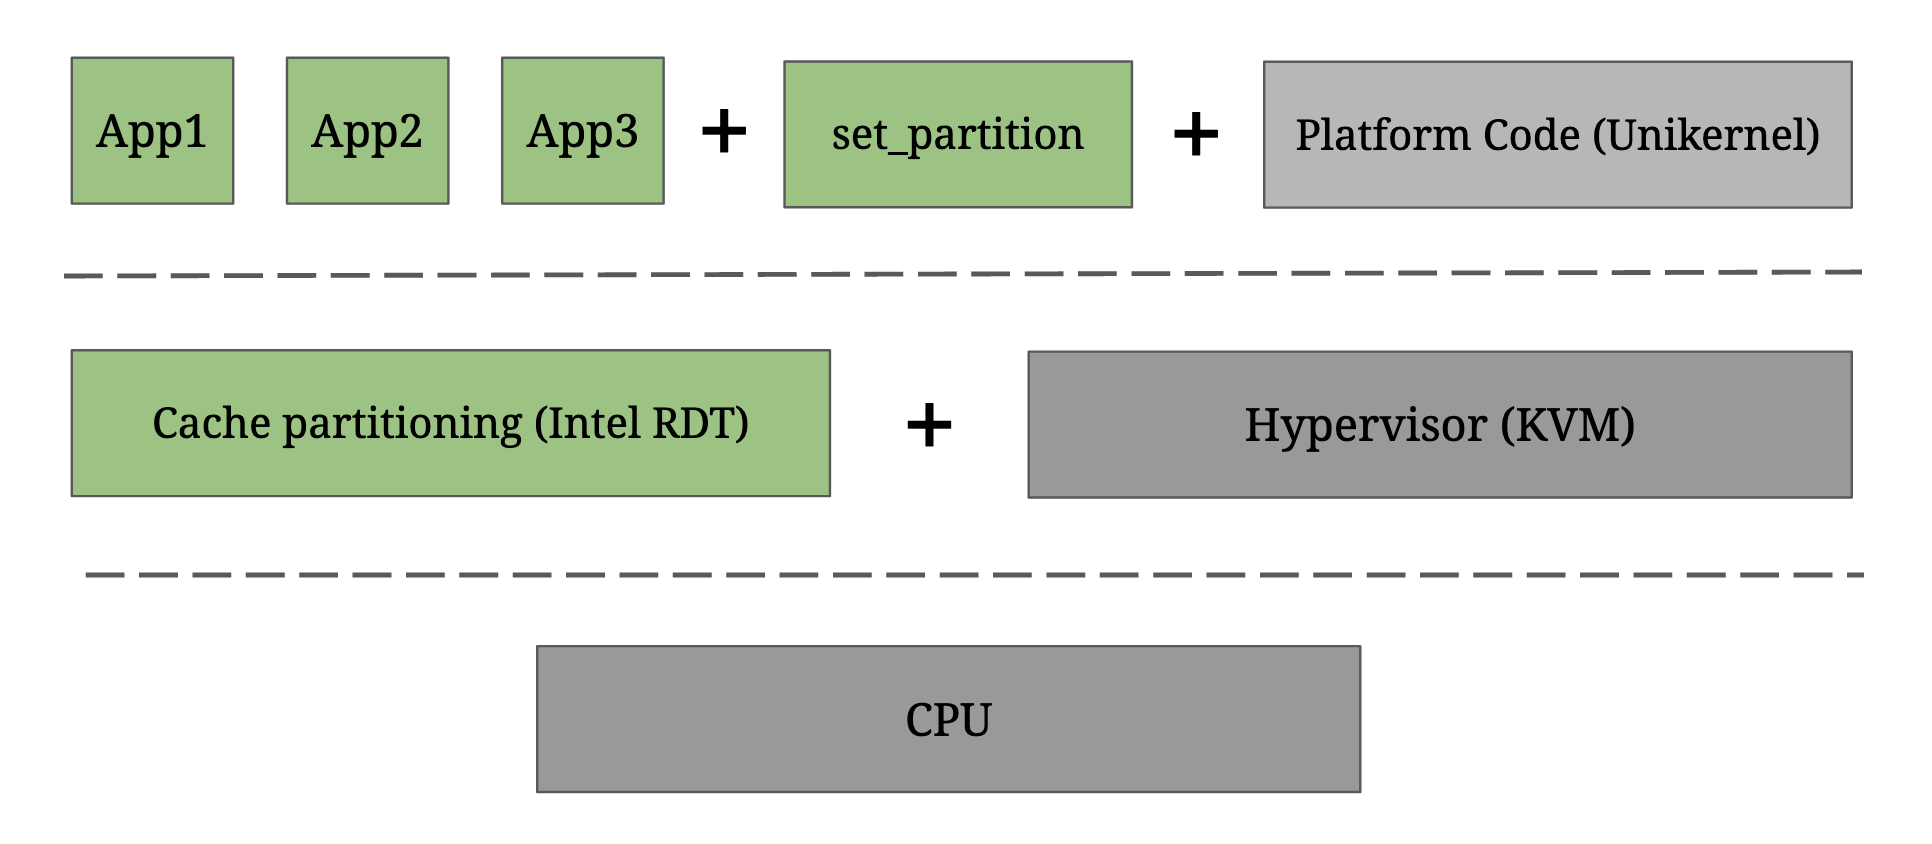
\includegraphics[width=\linewidth]{solution_architecture}
    \label{fig:solution}
    \caption{Solution architecture}
    \Description{Brief representation of our contributions at different layers.
    Boxes in green represent our contribution and boxes in grey are the existing
    systems that are being reused}
\end{figure}

We provide an overview of our solution architecture in Fig.2. The boxes in green
represent our own contribution and the grey boxes represent the existing
components that we have reused. We start with the description of the
$\texttt{set\_partition}$ application programming interface (API). The
application has access to an intrinsic function called
$\texttt{set\_partition(int partition\_id)}$. This allows it to denote an
abstract level for each section of the program. We expect the programmer to
instrument their applications with calls to this function using different
partition ids to denote which section the program is executing in. For example,
a programmer may denote the networking parts of their application to execute in
cache domain 1 and computational parts of their application exeucte in cache
domain 2. Since these identifiers are abstract, the application can decide the
scheme it uses to partition the application. A simple partitioning scheme would
be to demarcate all network IO into a certain partition and the rest of the
applications into another. Further refinements could even create paritions
within the networked section for more fine-grained control. Internally, this
intrinsic function is implemented as a hypercall in the hypervisor. A hypercall
is a mechanism for the user program to signal to the hypervisor that it needs
access to a special resource. This hands over control to the hypervisor which
performs the necessary operations to hand over control of the resource and
returns to the user program. Next, we describe the unikernel library - Unikraft,
that we use to turn our programs into unikernels. A unikernel library is a
specialized library that provides the necessary platform code to turn an
application in a bare-metal kernel. Thus, this kernel can now directly execute
on hardware (though it requires a hypervisor to provide some basic platform
abstractions). The advantage of this approach is that only the necessary code
needed to run the application is pulled into the final application binary. Thus,
since we do not need virtual memory, scheduling, IO emulation and other such
features, this code is not present in the kernel and thus the memory footprint
of these features is avoided. Unikraft \cite{unikraft} is a library OS, that
provides the necessary platform code and a build system to turn regular
applications into unikernels. These unikernels can be executed on a variety of
hypervisors such as KVM and Xen. It has implementations of standard POSIX
compatible syscalls and additional libraries can be ported to the Unikraft
environment for additional features. All the applications that we wrote for
performance evaluation were turned into unikernels using Unikraft and then
executed on a hypervisor. We also had to port additional libraries to support
our applications. Next, we provide details of the KVM hypervisor and how we
integrated our cache partitioning scheme into the hypervisor. There are two
types of hypervisors, Type-I and Type-II hypervisors. Type-I hypervisors run
directly on the CPU and provide isolation and platform abstraction features.
Type-II hypervisors are intergrated with an existing operating system and
re-uses the features of the operating system to provide platform abstraction.
Both types of hypervisors use hardware virtualization to provide isolation and
fast emulation of platform features. In our setup, we have used the KVM
hypervisor, which is integrated with the Linux operating system and uses Intel
VT-d to provide hardware virtualization. KVM has support for intercepting
hypercalls from guest kernels that it is running. It is in this subsystem that
we implement our cache-partitioning feature. We implement a new hypercall,
intercepts calls to $\texttt{set\_partition}$ from the guest OS. Then, we
inspect the domain ID provided by the guest OS and use it to allot it to a cache
partition. An important nuance to keep in mind is that the guest OS may be
executing on a different hardware thread than where the hypervisor intercepted
it. Thus it is important to use the features of KVM to signal the correct core
to allot the cache partition.

\begin{figure}[h]
  \centering
  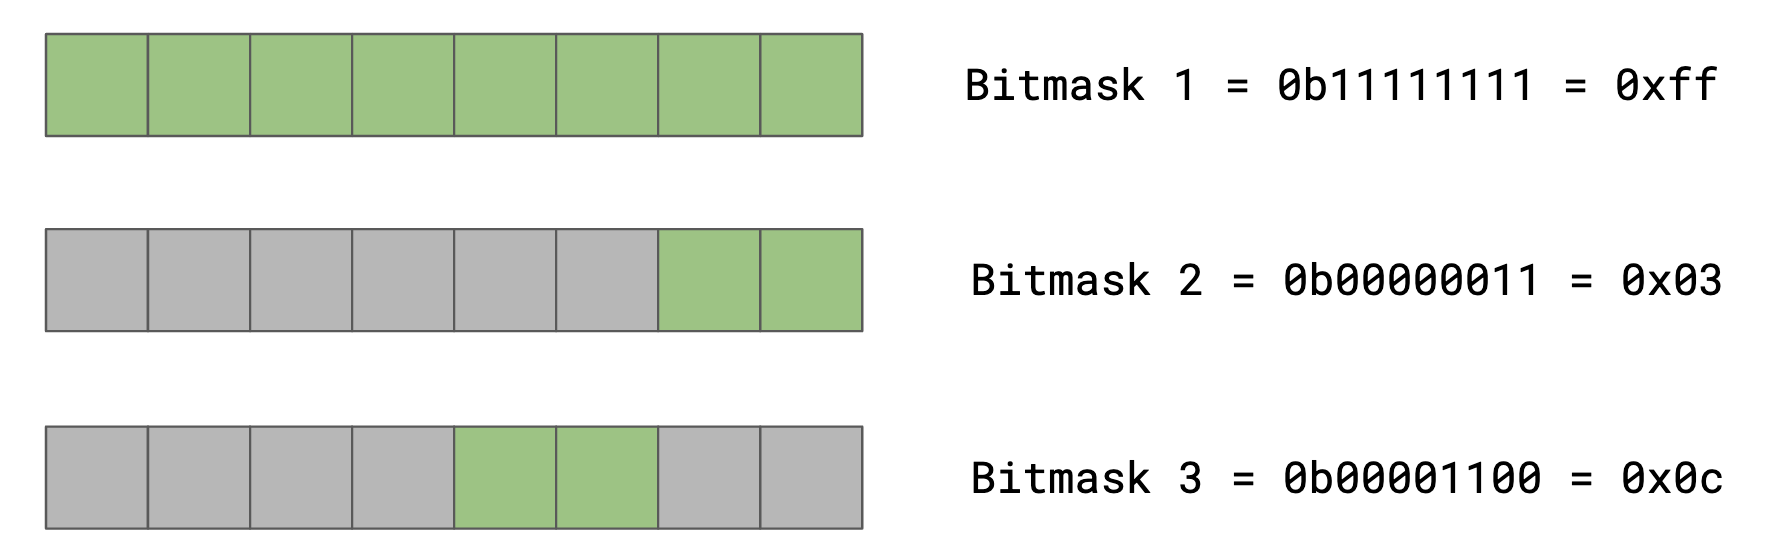
\includegraphics[width=\linewidth]{bitmasks}
    \label{fig:bitmasks}
    \caption{Example of cache bitmasks}
\end{figure}

Finally, this allotment is performed using the Intel Resource Director
Technology (RDT). Intel RDT has subfeature called Cache Allocation Technology
(CAT) which is a hardware feature that allows application level cache
partitioning. The first key component of CAT is the cache bitmask. A cache
bitmask is a fixed size bitstring that is used to represent the regions of the
cache that the application may occupy. We show some examples of bitmasks in
Figure 3. As can be seen, a 1 represents a cache region that an application may
occupy whereas a 0 represents a region it cannot. Thus, Bitmask 1 represents
access to the full cache and Bitmasks 2 and 3 to smaller sections of it. Notice
that Bitmask 2 and 3 are non-overlapping, thus applications execute under these
bitmasks will not interfere with the cache footprint of each other. Each
processor supports a fixed number of bitmasks to be preprogrammed in the system.
Once this is done, we can write a model-specific register in each logical core
which denotes which bitmask the current application should run under. This has
the effect of partitioning the cache such that the requests from the core now go
to the specific cache partition. We use this feature to dynamically switch cache
partitions whenever an application requests a $\texttt{set\_partition}$ call.


\section{Evaluation and Results}

The evaluation of our implementation requires careful analysis because there are
two competing effects at play. On one hand, partitioning cache space for the
networking parts may improve the effectiveness of DDIO by preventing the
eviction of RX/TX buffers. But on the other hand, this may reduce the cache
space available for the remaining parts of the application. Thus, even though
the performance of the networking parts improves the overall application
performance may suffer. Moreover, since our dynamic cache partitioning scheme is
implemented using hypercalls in an hypervisor, there is an overhead associated
with the VM exit. Thus, if these events are too frequenct, it may add a
non-negligible overhead leading to an increase in runtime. Given this, it would
not be possible to determine the impact of our work by simply measuring
wall-clock time. While an improvement in wall-clock time is great, it does not
provide any insight into which part of our solution resulted in this
improvement. In the case that performance is reduced, we need a method of
diagnosing what led to the decrease in performance. Thus we use hardware
performance counter events to benchmark different aspects of an application
which we believe capture the performance of our implementation. First, we focus
on PCIE Writes / Reads from the last level cache (LLC). This is the primary
event that identifies if our solution is working. This event provides
information about the number of PCIE accesses that were serviced from the LLC.
This is important because if we are servicing more requests from the LLC, this
implies that more network packets are staying resident in the cache and directly
being processed from there, instead of being retrieved from main memory. Second,
we focus on the total LLC Misses in the application. This is important because
by partitioning the cache there is a chance we increase the number of cache
misses in the application. Thus, we would like to analyze if the total number of
application cache misses is increasing substantially. Finally, we also measure
application level benchmarks such as bandwidth and latency of requests served,
since finally any improvement in the software should result in an observed
improvement in the client side performance. We present our results and discuss
our observations below.

\section{Related Work}
The work most closely related to our work is \cite{alireza_2020}. The work
performs a substantial analysis of the Intel DDIO implementation. Their
experiments consider different types of applications executed under different
cache partitioning schemes. The major takeaway from their work that we
capitalized on was that there is no \textit{one-size-fits-all} cache
partitioning policy. Thus we implement a solution that allows an application to
customize its use of the cache, tailored to its specific needs. On the front of
fine-grained cache-partioning, there are two main directions - software based
cache partitioning based on colored pages \cite{herter}, \cite{sherwood} and
hardware based way partitioning (such as Intel RDT) \cite{chen}, \cite{assaf}.
The work closest to our implementation is \cite{swap}, which also proposes a
fine-grained cache partitioning scheme. But their work does not consider the
effect of this scheme on networked applications. Further the implementation is
not performed using Intel RDT (which is a more mainstream implementation of
hardware cache partitioning) and also does not take into the effect of
hypervisor (necessary for safe isolation of applications).

\section{Future Work}

\begin{acks}
    To Prof. Muhammad Shahbaz for conducting such a great course and Sharuna
    Anandraj, Darwin Kamanuru, K M A Solaiman and Kai Ling for helping out
    throughout the semester!
\end{acks}

%%
%% The next two lines define the bibliography style to be used, and
%% the bibliography file.
\bibliographystyle{ACM-Reference-Format}
\bibliography{db}


%%
%% If your work has an appendix, this is the place to put it.
\appendix

\section{Contributions}

\subsection{Jiangqiong Liu}
Worked on the handling the measurement across the entire project. Implemented
perf scripts to automate collection of hardware counter events for all
applications and perform the post-processing to report the results. Correlated
performance changes in application based on measurement results.

\subsection{Joshua Reprogle}
Implemented an end-to-end Websocket server in C++ and used it to implement a
chat server. The C++ server was written without dynamic memory allocation to
carefully control the placement of memory buffers. Identified networking parts
of the application and performed $\texttt{set\_partition}$ instrumentation.

\subsection{Vedaant Rajoo}
Implemented a replicated, in-memory key-value store using C++. Analyzed
networking and computational parts of the application and performed
$\texttt{set\_partition}$ instrumentation.

\subsection{Sowmya Jayaram Iyer}
Implemented machine learning models for packet based classification. Executed
these models on real-world traces and ported them to run as Unikraft kernels.
Identified the $\texttt{set\_partition}$ instrumentation points for compute
bound parts of the application.

\subsection{Keerthana Ashokkumar}
Designed and implemented a replicated, in-memory key-value store using Java.
Implemented two phase commit based atomic updates and leader server replication.
Assisted in the C++ implementation of the in-memory store and identified
networking parts of the application.

\subsection{Anmol Sahoo}
Designed and implemented the Intel RDT based cache partitioning scheme as a KVM
patch in the Linux kernel. Exposed the userspace API as VMCALLs in KVM. Ported
the necessary libraries to Unikraft (rpclib for rpc, tcp/ip for sockets, tvm for
deep learning / machine learning). Performed end-to-end execution and testing of
all applications.

\end{document}

\endinput
%%
%% End of file `sample-sigconf.tex'.
